\documentclass[en]{../../../eplsummary}

\usepackage{../../../eplcode}

\usepackage{graphicx}
\usepackage{booktabs} % for much better looking tables
\usepackage{array} % for better arrays (eg matrices) in maths
\usepackage{paralist} % very flexible & customisable lists (eg. enumerate/itemize, etc.)
\usepackage{verbatim} % adds environment for commenting out blocks of text & for better verbatim
\usepackage{subfig} % make it possible to include more than one captioned figure/table in a single float
% These packages are all incorporated in the memoir class to one degree or another...
\usepackage{framed}
\usepackage{color}
\usepackage{multicol}

\hypertitle{Concurrent system theorical part}{7}{INGI}{2143}
{Nicolas Houtain\and Gorby Nicolas Ndonda Kabasele}
{Charles Pecheur}

\section{Question 1: LTS and Sequential processes}

\textit{Define labelled transition systems  and explain their underlying
assumptions. Using small examples, describe how sequential processes are
modelled in FSP (sequences of actions, termination, loops, choices, non-
determinism).Explain how data values are handled in FSP.}

\paragraph{}

\textbf{LTS} are finite state machine  with labels on  transitions that
define  a process,  each  state  of the  automata  represents the  state
the  process (value of  implicit/explicit variables,...).

\begin{tabular}{p{3cm}m{9cm}}
    \textsc{Assumption} =
    & \begin{enumerate}
         \item each action are atomic (do not interrupt each other).
         \item State are opaque (no info on the value, variable, register, memory...)
         \item Transition are transparent.
     \end{enumerate}
    \\
\end{tabular}


Executions of the process are finite or infinite, and this is a sequence
of  successive transitions  from the  \textit{initial state}.  (There is
different transitions for the same action)

As  the  process  execute,  it execute  statement  (atomic  action  like
read/write  in the  register). Each  action  in the  process, trigger  a
transition from the current to the corresponding state in the LTS.
FSP is the language used to model Finite State Process. Every Finite
State Machine can be model with FSP.

\paragraph{Example} for the FSP

\begin{lstlisting}
// Sequence
MEETING = (hello->converse->goodbye->END).

// Determinist choice
DRINKS = pay-> (coffee->DRINKS|tea->DRINKS).

// Non-determinism
DRINKS_ND = (pay->coffe->COINS|pay->tea->COINS).

// Loop + data handling
BUFF = (in[i:T]->STORE[i]),
STORE[i:T] = (out[i]->BUFF).
\end{lstlisting}
For different data values, different actions are done (in.0,in.1,...) . The range of the data values is finite. With
syntaxic sugar, we use indexing to represents implicit choice between indexes.


\section{Question 2: Concurrent process}

\textit{Explain  the model  of concurrency  used in  labelled transition
systems.  State  the  underlying   assumptions.  Using  small  examples,
describe  how  concurrent interacting  processes  are  modelled in  FSP.
Discuss how direction of interaction and data transfer is modelled.}

\paragraph{}

The model of concurrency used by LTS is \textbf{temporal ordering of event}. Two
actions are concurrenct  if they are no defined order  in which they can
occur,  ($a\to b$  or $b\to  a$). It  doesn't describe  the time  needed
for  a  event  to  finish  and  how  long  is  the  delay  between  each
event. (Concurrency  can be described  as choice because  of scheduling)

\begin{tabular}{p{3cm}m{9cm}}
    \textsc{Assumption} =
    & \begin{enumerate}
         \item Action are atomic, Transitions occur instantaneously
         \item Process execute at arbitrary speeds
         \item Action are  interleaved (does not model the  case where a
               and b occur simultanously)
     \end{enumerate}
    \\
\end{tabular}

\paragraph{Interleaved} is not a problem because of \textit{no partial overlap}
(assumption\#1) and when occu at the same time then they can also occur consecutively
(assumption\#2).

$ \rightarrow $ Occur same time does not affect our model of concurrent executions


\paragraph{FSP}
Compose concurent processes with \textit{Disjoin Parallel Composition} ($||$).
LTS generate this by combining LTS from sub-processes.


\paragraph{ } Concurrency ca be described as \textit{choice} by scheduling


\paragraph{Example} for the FSP

\begin{lstlisting}
// Basic concurrency
ITCH = (scratch->STOP).
CONVERSE = (think->talk->STOP).
||CONVERSE_ITCH = (ITCH || CONVERSE)

// Shared action
MAKER = (make->ready->MAKER).
USER =(ready->use->USER).
||MAKER_USER = (MAKER || USER)

//
\end{lstlisting}

The concurrent model is a cartesian product between the set of action of
each process.

\begin{itemize}
    \item \textit{Disjoint} action are interleaved
    \item \textit{Shared} action are synchronized
\end{itemize}
In  our  example,  it  means that  to  do  \textit{ready},  the
concurrent process must have done a \textit{make} first.


\paragraph{Discuss data transfert }
For different data values, different actions are done (in.0,in.1,...) . The range of the data values is finite. With
syntaxic sugar, we use indexing to represents implicit choice between indexes.


\section{Question 3: Hiding relabelling,priority}


\textit{Using  small  examples,  describe the  relabelling,  hiding  and
priority operators of FSP.Explain the  semantics of hiding, its relation
to  abstraction, and  how  this abstraction  helps  in verifying  large,
complex models.}

\paragraph{ }

Example FSP
\begin{lstlisting}
// Relabeling
CLIENT = (call->wait->continue->CLIENT).
SERVER = (request->service->reply->SERVER).
||CLIENT_SERVER = (CLIENT || SERVER)/{call/request,reply/wait}.

// Hiding
BUFF = (in[i:1..1]->out[i]->BUFF).
||TWOBUF = (a:BUFF||b:BUFF)/{in/a.in,a.out/b.in,out/b.out}
							    \{a.out}.
// Priority
PROGRAM =(work->write->PROGRAM).
PRINTER = (read->print->PRINTER|sleep->PRINTER).
||SYSTEM = (PROGRAM || PRINTER)/{transfer/{write,read}}
				<<{transfer}.
\end{lstlisting}

\begin{description}

    \item[Relabeling] allow proccesses  to \textit{share} common action.
    It's use  to make  the different process  synchronize on  the action
    relabeled (explain client-server).
    $$ \textrm{ PROCESS / \{newname/\{oldname1, oldname2 \} \}} $$

     \item[Hiding] (like a abstraction) allow  process to make an action
    invisible  from  outside,  the  process  become  like  an  interface
    (explain the two buffer). If an action is hidden, it is replaced by a
    internal action \textit{tau}.
    $$ \textrm{PROCESS \textbackslash \{action1, action2 \} (hidden action) } $$
    $$ \textrm{PROCESS @ \{action1, action2 \} (show only action) } $$

    \item[Priority] allow process  to know which it  should priority to.
    (\textit{P$<<$A gives A high priority than P}).

        If A has  a high priority, whenever an action A  is enabled other
    action are disabled  including \textit{tau} (if the  process have to
    do a choice, it will take A)

\end{description}

\paragraph{Abstraction}
Hiding is an abstraction because the process becomes like a black box where internal action are hidden from
the outside.
\subparagraph{tau} is never a part of the alphabet, and no synchronize.
(minimise to eliminate it)

\subsection{Hiding semantic}
Hiding $B \subset Act$
\begin{itemize}
    \item $\alpha(E \backslash B) = (\alpha(E) - B)$
    \item $end(E \backslash B) = end(E)$
\end{itemize}
$$ \frac{E -a \to E'}{E\backslash B -\tau \to E'\backslash B} a\in B \quad \textrm{ and } \quad  \frac{E -a \to E'}{E\backslash B -a \to E'\backslash B} a\notin B $$


\section{Question 4: Semantics traces}

\textit{State the three key elements that constitute a formal semantics.
Define  those elements  for  the  trace semantics  of  FSP. Discuss  the
limitations of using finite traces as a semantics for FSP}

\paragraph{}
The three key elements are the following:
\begin{enumerate}
\item semantic domain \textbf{Dom}, represent the meaning of FSP programs (Trace or LTS)
\item semantic map \textbf{sem} from an $Exp \to Dom$
\item semantic relations $\leftrightarrow$ that defines relation over Dom (ex: equivalence, preorder, \ldots). Gives a semantics to every program
\end{enumerate}

\begin{figure}[h]
    \centering
    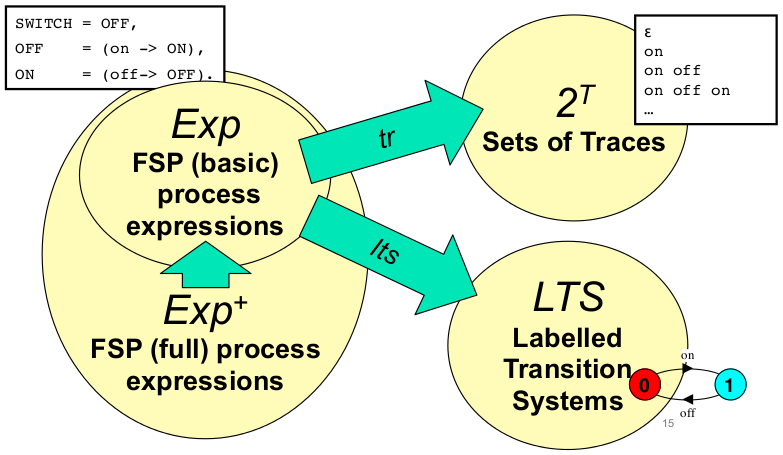
\includegraphics[width=10cm]{semantic.png}
\end{figure}

\begin{description}
    \item[Act] : universal set of \textbf{observable actions} (infinite)
    \item[tau] : $\tau \notin Act$. All actions = $Act \cup \{\tau\}$
    \item[Exp] is the set of all FSP (basic) process expressions.
    \item[Exp$^+$] is the set of all FSP (full) process definition
    \item[T = Act$^*$] is the set of all traces
    \item[2$^T$ ] is the set of all sets of traces
    \item[$\alpha$(E)] is the alphabet of processes
\end{description}

\paragraph{Trace  semantic}  is \textcolor{red}{TR}:  Exp  $\rightarrow$
2$^T$. A trace is a finite sequence observable actions.

TODO recursion and fixpoint


\paragraph{}
Trace semantics is limited for non-determinism and deadlock:
\begin{lstlisting}
// Non-determinism
P1 = (a->(b->STOP|c->STOP)).
P2 = (a->b->STOP|a->c->STOP).

// Deadlock
P3= (a->b->STOP).
P4= (a->b->STOP|a->STOP).
\end{lstlisting}

P1  and P2  have the  same  trace, while  they  are different  as P1  is
deterministic and P2  is not. Same result  for P3 and P4,  they have the
same trace but they are different as  P4 may deadloc after a. With trace
semantics, we can't distinguish between the two.
\section{Question 5: Semantics LTS}

\textit{State the three key elements that constitute a formal semantics.
Define  those  elements  for  the  LTS semantics  of  FSP.  Explain  the
principles of  structured operational semantic rules.  State and explain
the semantic rules for the choice and parallel operators.}

\paragraph{}
The three key elements are the following:
\begin{enumerate}
\item semantic domain \textbf{Dom}, represent the meaning of FSP programs (Trace or LTS)
\item semantic map \textbf{sem} from an $Exp \to Dom$
\item semantic relations $\leftrightarrow$ that defines relation over Dom (ex: equivalence, preorder, \ldots). Gives a semantics to every program
\end{enumerate}

\paragraph{Semantic map} for LTS is \textcolor{red}{lts}:Exp$\to<S,A,\Delta,q>$ where for process expression E:

\begin{itemize}
\item q is the initial state (=E)
\item A is the action set ($\color{red} \alpha(E) \color{black} \cup {\tau}$)
\item $\Delta$  is the transition relation  as a set of  \textcolor{red}{inference rules}
(set of premisse that lead to a conclusion)
\item Uses auxiliary map \textcolor{red}{end(E)} for sequential composition
\item S  is a  set of  state that contains  all the  states that  can be
reached from q through $\Delta$
\end{itemize}

To do the mapping  of an FSP process E, we  take this process expression
as initial state of our LTS (q=E).  A = alphabet(E) + tau. Delta defined
by set of  inference rules. Use auxiliary map end(E)  for composition. S
contains all states reachable from q through Delta.

\paragraph{Operational semantics}
Define transitions E -a $\to$ E' then derive $\Delta$

\subsection{An  inference rule}  is a  set  of rules  with the  following
form   :
$$\frac{\varphi_1,...,\varphi_n}{\varphi}\quad c, \quad \textrm{  which  means  } \mathbf{IF} \quad
\varphi_1,...,\varphi_n \quad [\mathbf{WHERE} \quad c] \quad \mathbf{THEN} \quad \varphi$$

In the LTS, $\varphi$ are the transitions $E - a\to E'$ and the premisses
$\varphi_1,...,\varphi_n$ are the transition of the subprocesses of E.

\subsection{stuctural operational semantics (SOS)}
Structured operational semantics rules define transition relations by induction of the syntax of language.

\subsection{Semantic rules}

\subsubsection{Choice}
The semantic of the \textbf{choice operator} is as follow:
\begin{itemize}
    \item $\alpha(E_1|E_2) = \alpha(E_1)\bigcup\alpha(E_2)$
    \item $end(E_1|E_2) = end(E_1) \vee end(E_2)$ = false because $E_1,E_2$ are guarder processes a->E
\end{itemize}

It is  based on the  two inference rules
$$\frac{E_1-a->E'}{E_1|E_2 -a-> E'} \quad \textrm{ and } \quad \frac{E_2-a->E'}{E_1|E_2 -a-> E'}$$

which state that if one of
the process can reach E', then the whole system can do it too.

\subsubsection{Parallel operators}

The semantic of the \textbf{parallel operator} is as follow:
\begin{itemize}
\item $\alpha(E_1|[A]|E_2) = \alpha(E_1)\bigcup\alpha(E_2)$
\item $end(E_1|[A]E_2) = end(E_1) \wedge end(E_2)$
\end{itemize}
It is based on three rules,
$$\frac{E_1-a->E'_1}{E_1|[A]|E_2->E'_1|[A]|E_2}a\notin A \quad \textrm{ and } \quad
\frac{E_2-a->E'_2}{E_1|[A]|E_2->E_1|[A]|E'_2}a\notin A$$
$$\textrm{ and } \frac{E_1-a->E'_1 \quad E_2-a->E'_2}{E_1|[A]|E_2->E'_1|[A]|E'_2}a\in A$$

where A = $\alpha(E_1)\bigcap\alpha(E_2)$

\section{Question 6: Equivalences LTS}

\textit{Explain  the notions  of equivalence  and preorder  relations on
concurrent models.  Define strong and weak  equivalences. Illustrate then
difference  between  trace and  weak  equivalence.  Give an  example  of
preorder relation based on LTS and discuss its usefulness.}

\paragraph{}  The equivalence  allow to  tell if  two FSP  processes are
equal.

\begin{figure}[h]
    \centering
    \begin{tabular}{c|lcr}
         $=_{FSP}$ & same FSP  \\
         $=_{LTS}$ & same LTS (isomorphic) \\
         $\sim$ & strong equivalence &:& \textit{There exists a strong bisimulation $R(E_1, E_2)$} \\
         $\approx_c$ & weak congruence &:& \textit{ }  \\
         $\approx$ & weak equivalence &:& \textit{there exists a weak bisimulation $R(E_1, E_2)$}\\
         $=_{tr}$ & same traces \\
    \end{tabular}
    \caption{Different type of equivalence, listed by order of restricivity}
\end{figure}

\subsection{Trace equivalence}

Given E, E'$\in$ Exp $$ E=_{tr}E'  \textrm{ \textcolor{red}{IFF} }tr(E) = tr(E')$$
$=_{tr}$ is a \textbf{equivalence} relation which means it's reflexive, symmetric, transitive.

\subsection{Trace preorder}
Given $E_s,E_i \in EXP$ $$E_i \le_{tr} E_s \textrm{ \textcolor{red}{IFF} } tr(E_i)\subseteq tr(E_s)$$
$\le_{tr}$ is a reflexive and transitive. $E_i$(impletmentation) is a refinement of $E_s$(specification)

\paragraph{Note:}
\begin{itemize}
    \item $=_{tr}$ ignores non determinism
    \item $\le_{tr}$ preseerves safety properties
    \item $\le_{tr}$ says nothing of liveness properties ($ STOP \le_{tr} E_s$)
\end{itemize}

\subsection{Simulation}
A process  P1 \textbf{simulates} a process P2 \textcolor{red}{IFF} it  covers all  the possible
behaviours of  P2, i.e :
\begin{enumerate}
    \item Any transition of P2, there is a corresponding transition that P1 can perform
    \item The states reached by P1 cover all the possible behaviours of the
        corresponding state reached by P2
\end{enumerate}

\textit{If P2 and P1 can simulate each other, they are in bisimulation.}


\paragraph{Pre-order}
Same idea that trace pre-order

\paragraph{Equivalence}
$E_1$ is (strong) simulation equivalent to
$$E_2 (E_1\asymp E_2) \quad \textrm{IFF} \quad E_1\prec E_2 \quad and E_2\prec E_1 $$


\subparagraph{ } It means that they can simulate each other but it's not
the same as  bisimulation equivalence. One $R(E_1,E_2)$ such  that R and
$R^1$ are both simulation (in  opposition of strong simulation where all
state of $E_1$ must simulate all state of $E_2$ )

\begin{figure}[h]
    \centering
    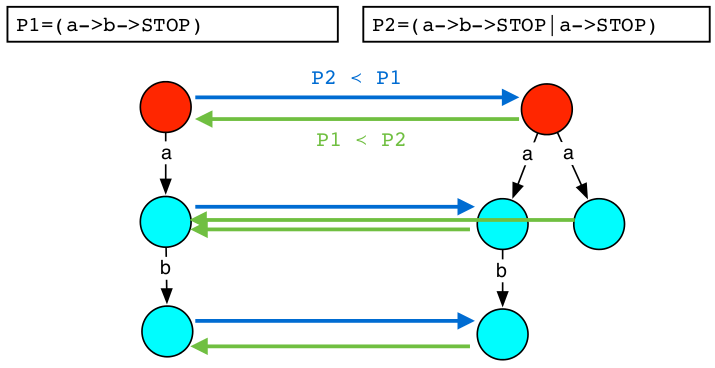
\includegraphics[width=8cm]{sim_equi.png}
    \caption{Simulation equivalence}
\end{figure}

\paragraph{Ready}
Ready simulation is a strong simulation with
$ if E_2 -a \to$ then $E_1 -a \to$

\begin{figure}[h]
    \centering
    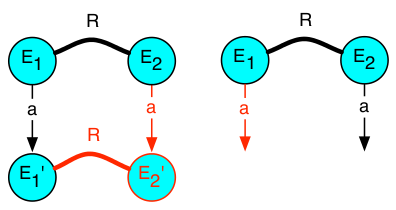
\includegraphics[width=6cm]{ready.png}
    \caption{Ready simulation}
\end{figure}

\subsubsection{Strong simulation}
Given $R \subset Exp \times Exp$ , for every $(E_1, E_2) \in R$
$$ \textrm{ \textcolor{red}{IF} } E_1 -a \to E'_1 \textrm{ \textcolor{red}{THEN} } E_2 -a \to E'_2 \textrm{ \textcolor{red}{AND} } (E'_1, E'2) \in R$$

\paragraph{     }     $E_2$    \textbf{strongly     simulates}     $E_2$
\textcolor{red}{IF}   each  $E'_2$   strongly   simulates  each   $E'_1$
\textcolor{red}{AND} $(E_1, E_2) \in R$

\paragraph{ } There where strong  bisimulation, when $E_1$ and $E_2$ are
both strong simulations.


\subsubsection{Weak transitions}
\begin{itemize}
    \item $E -a_1 \cdots a_n \to E'$ \textcolor{red}{IFF} there exists $E_0, E_1, \cdots, E_n$
        such that $E = E_0 -a_1 \to E_1-a_2 \to \cdots -a_n \to E_n = E'$

    \item $E = a \to E'$ \textcolor{red}{IFF} $E -\tau* a\tau* \to E'$ (for a$\in$Act)

    \item $E = \epsilon \to E'$ \textcolor{red}{IFF} $E -\tau* \to E'$
\end{itemize}

\subsubsection{Weak simulation}

Weak simulaton is  the same idea but it's less  restrictive as it ignore
the hidden action ($\tau$).

Given $R \subset Exp \times Exp$, for every $(E_1, E_2) \in R$, $t \in Act \cup \{\epsilon\}$
$$ \textrm{ \textcolor{red}{IF} } E_1 =t \to E'_1 \textrm{ \textcolor{red}{THEN} } E_2 =t \to E'_2 \textrm{ \textcolor{red}{AND} } (E'_1, E'2) \in R$$

\paragraph{Note about t} :
\begin{enumerate}
    \item $t = a \in Act$ : t = $\tau* a \tau*$
    \item $t = \epsilon$  : t = $\tau*$
\end{enumerate}

\subsection{Congruence}
A congurence $\zeta$ is an equivalence relation such that \textcolor{red}{IF}
$E \zeta E'$ \textcolor{red}{THEN} $C[E] \zeta C[E']$ for any context $C[\bullet]$


\textit{(Equals can be substituted for equals)}.

\subsection{Other}

\paragraph{Internal choice}
Non deterministic choice and deterministic choice are
NOT weakly equivalent, but are trace equivalent.


The difference between from weak equivalence and trace equivalence can come from non-determinism.

\paragraph{Divergence}
is a loop of internal actions. (Weak equivalence ignores divergences)


\subsection{Example}
The  example shows that  P1,P2,P3 are not  strongly equivalent
because the internal action are considered.

\begin{lstlisting}
P1 = (a->b->STOP).
P2 =(a->i->b->STOP)\{i}.
P3=(i->a->b->STOP)\{i}.
\end{lstlisting}

For  two  FSP  processes(=LTS   states)  $E_1,E_2$,  $E_1$  is  strongly
equivalent to  $E_2$ iff there exist  a strong bisimulation R  such that
$R(E_1,)$



\section{Question 7: Minimization}

\textit{Define  minimization modulo  an  equivalence.  Give the  general
principles of the coarsest partition algorithm. Discuss how minimization
can be performed in a compositional way.}

\subsection{Minimization modulo equivalence}

For a given   equivalence  relation eq  (ex:weak  bisimulation  equivalence
$\approx$) and a given LTS,  P :
$$ \textrm{ There is  a smallest LTS P'  such that P'  eq P } min(P) =  \textrm{min }{P'\quad | \quad P' \textrm{ eq
P} }$$

It is possible to construct  min(P), called minimizing P (modulo  eq). It can be
done by merging state and by removing some $tau$ transitions.

\subsection{Coarsest partition algorithm}

The goal of  the coarset partition algorithm is to  group all equivalent
states (according to eq). It constructs  equivalence classes and then buil
a partition of the state space. The algortihm works as follow:

\begin{enumerate}
    \item group all states(one single equivalence class)
    \item while some class X does not respect the equivalence relation
    \begin{enumerate}
        \item split non-equivalent states of X into different classes X1,...,Xn
    \end{enumerate}
\end{enumerate}

\begin{figure}[h]
    \centering
    \begin{tabular}{cc}
        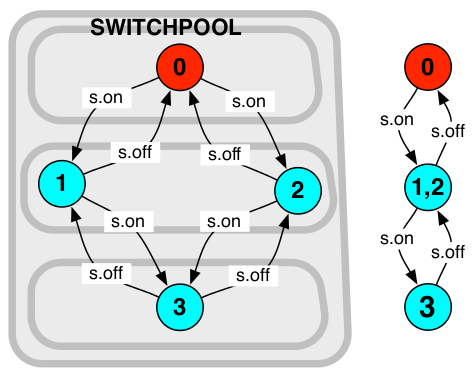
\includegraphics[width=7cm]{strong_mini.png}
        &
        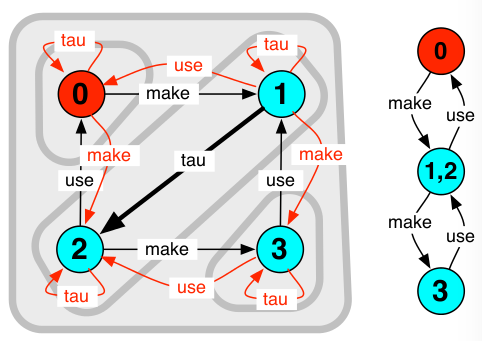
\includegraphics[width=7cm]{weak_mini.png}
        \\
    \end{tabular}
    \caption{Example of strong and weak minimization}
\end{figure}

\textbf{Tau closure} is the principle used to do a minimization based on
weak equivalence, the principle is as follow:

\begin{itemize}
\item add E\textcolor{red}{-a} $\to$  E' for every E-$\tau a\tau* \to$E'
\item add E $\color{blue}{-\tau \to}$ E' for every E-$\tau* \to$ E'
\item Then apply strong equivalence.
\end{itemize}

\subsection{Compositional Minimization}

\begin{tabular}{m{11cm}m{4cm}}
Given a composite FSP E with component $E_1,...,E_n$. & \\
\begin{enumerate}
\item Generate LTS $P_i=lts(E_i)$
\item Minimize LTS $P'_i=min(P_i)$
\item For each composite FSP $E_k=(E_i||E_j)/R\backslash A$
\begin{enumerate}
\item Genrerate LTS $P_k = (P'_i||P'_j)/R\backslash A$
\item Minimize $P'_k=min(P_k)$
\end{enumerate}
\item Analyze $P'_n$ where $E_n=E$
\end{enumerate}
&
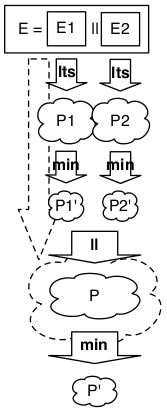
\includegraphics[width=2cm]{minimization.png}
\\
\end{tabular}

$\rightarrow$ \textcolor{red}{Gain} : $|P'|<|P|<|lts(E)|$

It means  that it is more  effiecent to do mimizing  in hierarchical way
and not  only at  the end because tau closure are really costly.  There is no usefulness to minimize different part of the system if there is no
syncronization.

(remember ABSTRACT in the project + example) slide 56 chap 5).

\begin{lstlisting}
// No sync
minimal ||NODES = (a:NODE||b:NODE)
minimal ||CHANNELS = (ab:CHANNEL || ba:CHANNEL)
minimal ||SERVICE = (NODE||CHANNELS) /R \A

// Sync
minimal ||NODE_CHAN_A = (a:NODE || ab:CHANNEL) / R \A
minimal ||NODE_CHAN_B = (b:NODE || ba:CHANNEL)
minimal || SERVICE = (NODE_CHAN_A || NODE_CHAN_B) /R \A
\end{lstlisting}


\section{Question 8: Synchronizarion models}

\textit{Using   small    examples,   illustrate   how    the   following
synchronization mechanisms can  be modeled in FSP  : rendez-vous, shared
variables,  locks,  semaphores,  buffers.  Explain the  notion  of  data
independence.}

\subsection{Synchronization mechanism}
\begin{lstlisting}
// Rendez-vous
MAKER = (make->ready->MAKER).
USER = (ready->use->USER).

// Shared variable as an explicit separate process
const N = 2
range T = 0..N
VAR = VAR[0],
VAR[u:T] = (read[u] -> VAR[u] | write[v:T] -> VAR[v]).

// Lock
LOCK = (acquire->release->LOCK).

// Semaphore
const Max = 3
range Int = 0..Max
SEMAPHORE(N=0) = SEMA[N],
SEMA[v:Int] = (up->SEMA[v+1])
			|when(v>0) down->SEMA[v-1]),
SEMA[Max+1] = ERROR.

// Buffer, use many instance to make a table of buffer
//or a channel if they communicate with each other
range T = 0..2
BUFFER1 = (in[x:T] -> out[x]->BUFFER1).
\end{lstlisting}

\subsection{Mecanismes}

\subsubsection{Rendez vous}
Actions occur in all paricipating processes (\textit{synchronous}),
so some processes are blocking to wait other processes are ready to
perform the action.

\textit{Unless it has the choice to perform an alternative action}

\paragraph{Synchronous message passing}
Like sender/receiver.

\subparagraph{Determined data value}
P[x:Data] = ( c[x] $\to$ P1[x]).

\subparagraph{Undetermined data value}
Q = (c[x:Data] $\to$ Q1[x]).


\subsubsection{Shared variable}
is modeling in FSP by an explicit separate process.

\subsubsection{Lock}
is modeling in FSP by an explicit separate process.
(Example pg 75)

\subsubsection{Monitor}

A   monitor   is   a   construct   for   concurrent   programming   with
\textit{encapsulated  data}, \textit{mutual  exclusion}, \textit{monitor
procadure calls} (that can blok until a given condition is satisfied).

\paragraph{In FSP} :
\begin{itemize}
    \item Procedure calls are represented as signe actions
    \item Condition synchronization by enabled/disabled action
    \item Data/state encapsulation is built-in
\end{itemize}

\subsubsection{Semaphores}
Like a monitor but the condition is non-negative integer
variable.

\subsubsection{Buffer}

\subsection{Data independence}

If the  medium which carries the  data change it or interprete it, the
number of state can become quite large.  But if it's not affected by the
precise value being transmitted the system is \textbf{data-independent}
(\textit{The data can be abstracted away often resulting in simpler models})

\paragraph{Example :} Bounded buffer becomes a bounded counter

\section{Question 9: Timed systems}

\textit{Explain how timed systems can be modeled in FSP and what are the
underlying assumptions. Give a small example. Define the notions of time
consistency and maximal  progress and discuss how  they occur concretely
in FSP models}

\subsection{Time in FSP}
We can use clock as a mean of synchronization to model timed system.

\begin{tabular}{p{3cm}m{9cm}}
    \textsc{Assumption} =
    & \begin{enumerate}
          \item Program execution is negligible with respect to external events. (action take zero time to be executed)
          \item No assumption on duration, relative speed (only ordering of event)
          \item Instantaneous processing
     \end{enumerate}
    \\
\end{tabular}


Even if real time is continuous, we use a \textit{discrete model} of time in FSP.
We  use the  \textbf{ticks}  of a  clock  and the  time  is measured  by
counting the ticks.
\textit{The time between two ticks is a fixed duration d.}

\begin{figure}[h]
    \centering
    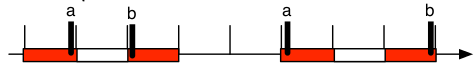
\includegraphics[width=8cm]{timing.png}
    \caption{timing uncertainty}
\end{figure}

$\rightarrow$ The accuracy  of  time  measurement can  be
increased  by reducing  the value  of  d but  the  price to  pay is  the
increase of the number of state.

\paragraph{Timed systems in FPS}
\begin{enumerate}
    \item Choose one action to represent clock transition (\textit{tick})
    \item All time-dependent processes synchronize on \textit{tick}
    \item Time-indepedent processes do not use \textit{tick}
\end{enumerate}


\subparagraph{Deadlock}
is when time is blocked, i.e \textit{tick} cannot occur

\paragraph{Example}

\begin{lstlisting}
// Double click
DOUBLECLICK(D=2) = (tick->DOUBLECLICK|click->PERIOD[0]),
PERIODE[t:0..D]= (when (t==D) tick -> DOUBLECLICK
                    |when(t<D) tick->PERIODE[t+1]
                    |click -> doubleclick -> DOUBLECLICK ).
\end{lstlisting}


\subsection{Time consistency}
is a \textbf{global model property} and is not a requirement on individual processes

\begin{itemize}
    \item \textbf{A time-stop} is a deadlock in a timed model
    \item If no time-stop can occur in a timed model, then it's \textbf{time consistent}.
\end{itemize}

\begin{lstlisting}
CONSUMER(Tc=3) = (item->DELAY[1]|tick->CONSUMER),
DELAY[t:1..Tc]= (when(t==Tc) tick ->CONSUMER
				|when(t<Tc) tick->DELAY[t+1]).

PRODUCER(Tp=3) = (item->DELAY[1]),
DELAY[t:1..Tc]= (when(t==Tc) tick ->PRODUCER
				|when(t<Tc) tick->DELAY[t+1]).
\end{lstlisting}
The deadlock occur with Tc=2 and Tc=3, because after the first item is produced and accepted by the
consumer, the producer tries to produces another item after two clock ticks while the consumer must accept
a third to accept the item.

\subsection{Maximal Progress}

\begin{itemize}
 \item Action occur as soons as all participants are ready to perfom them.
 \item In FSP that all actions than can occur will occur before the next tick

     ($\rightarrow$ it can be done by giving a low priority to the tick action).
\end{itemize}

\paragraph{Infinite executions}
With the low priority at \textit{tick} it's possible to never make tick..

Resolve with \textbf{fairness}

\section{Question 10: Properties safety}

\textit{Define  and compare  deadlock, safety  and liveness  properties.
Discuss how deadlocks can appear in concurrent systems, and how they can
be remedied.  Using a small  example, explain how safety  properties are
modeled in FSP. Explain the  general technique used for verifying safety
properties.}

\subsection{Definition and comparaison}
\label{property_definition}

\begin{description}

    \item[deadlock  :] A  deadlock state  is  a state  with no  outgoing
        transition.
        \begin{itemize}
            \item state  q sat  \textbf{deadlock} \textcolor{red}{IFF} q'
            there exists no a, such that q-a$\to$                                q'
        \end{itemize}

    \item[Safety properties  :] \textcolor{red}{bad}  things don't  happen (violate  if a
        \textit{finite} path where bad thing happen)

    \item[Liveness  propeties :]  \textcolor{red}{good} things  do happen  (violate if  a
        \textit{infinite} path where no good thing happens)
\end{description}


Safety properties are  more of a protection on the  model while liveness
properties are more of an assurance on what the model do. \textbf{Both of
them  are  path properties}.  What  we  mean  by  bad things,  it's  the
condition on the succession of states and action along the path.


\subsection{Deadlock in concurrent system}

There can be deadlock in concurrent if the different parts of the system
share  ressources.  There can  be  deadlock  \textcolor{red}{IFF} the  following  four
conditions holds:

\begin{enumerate}

    \item \textbf{Serially reusable  resources :}  the processes  involded share
    resource which they use under mutual exclusion

    \item \textbf{Incremental  acquisition :}  processes  hold  on to  resources
    already  allocated  to  them  while waiting  to  acquire  additional
    resources

    \item \textbf{No pre-emption :} once acquired by a process, resources cannot
    be pre-empted(forcibly withdrawn) but  are only released voluntarily

    \item \textbf{Wait-for  cycle :}  a  circular chain(or  cycle) of  processes
    exits such that each process holds  a resource which its succesor in
    the cycle is waiting to acquire.

\end{enumerate}

\paragraph{They can be remedied by} :
\begin{enumerate}
    \item using different structure(semaphore, lock, ...) to protect the resource
    \item using timeout to avoid deadlock
    \item break the cycle (like philosophers)
\end{enumerate}

\subsection{Example}

Example of a safety property
\begin{lstlisting}
    propety POLITE = (knock->enter->POLITE).
\end{lstlisting}
The property state that two successive enter or knock can not happens.

\subsection{Verifiying}

To verify a safety propety, a \textbf{breadth-first search} is used. The
following situation are reported by the verification:

\begin{itemize}
    \item deadlock state
    \item error states (=ERROR, state that violates the property)
    \item (not END states)
\end{itemize}

\section{Question 11: Properties liveness}

\textit{Define  and compare  deadlock, safety  and liveness  properties.
Explain why  the technique used  for safety verification cannot  be used
for liveness verification. Explain the notion of fairness. Using a small
example,  explain  the  what  FSP's progress  properties  are,  and  the
technique used for verifying those properties}

\subsection{Definition and comparaison}
See \ref{property_definition} page \pageref{property_definition}

\subsection{Verification technique}

The verification  technique used  for safety  property (reachability) is
not enough to verify liveness properties as \textbf{the violation trace
are infinite}. Indeed, for a finite prefix, the good thing may not have
happened yet.

\subsection{Fairness}

Fairness  is  a property  which  assure  that for  a  set  of action  A,
each  action  will always  eventually  be  executed. It's  the  opposite
of  \textbf{starvation}.  It  is  often  based  on  \textbf{Fair  choice
Assumption}, which state  that if a choice over a  set of transitions is
executed  infinitely often,  then every  transition in  the set  will be
executed infinitely often.

\subsection{Verification on progress}

A progress state  that in infinite execution, assuming  fair choice, and
action will  occur infinitely  often, for the  example below,  the first
progress is  respected but not the  second one because, there  is a case
when no tails can be done.

\begin{lstlisting}
TWOCOIN = pick->COIN|pick->TRICK),

// Normal coin
COIN = (toss -> heads COIN|toss-> tails -> COIN),
// Trick coin
TRICK = (toss->heads->TRICK).

progress HEADS = {heads}
progress TAILS  ={tails}
\end{lstlisting}

The  verification  is  done  by  using  the  \textbf{Strongly  Connected
component(SCC)} and terminal set of a LTS P.

\begin{description}

    \item \textcolor{green}{The SCC of P} is a maximal  set of state S' $\subseteq$ S such
    that for all q, q' in S', q' is reachable from q.

\item \textcolor{red}{A terminal set of P} is  a SCC S'$\subseteq$ S such that there
    is no q in S', q'' outside S' such that q' is reachable from q.
\end{description}

\begin{figure}[h]
    \centering
    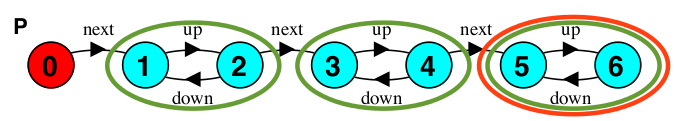
\includegraphics[width=10cm]{terminal.png}
    \caption{SCC and terminal set}
\end{figure}

 The  verification is  done as  follow give  a model(LTS)  and a  set of
 progress properties $A_i$ with $A_i \subset Act$:

\begin{enumerate}
    \item Search for all terminal set of states $S_T$
    \item Check that at least one action from every progress property $A_i$ occurs in each terminal set $S_T$
    \item if some $A_i$ does not occur in some $S_t$, report:
    \begin{itemize}
        \item the shortest path to $S_T$
        \item the action occuring in $S_T$
    \end{itemize}
\end{enumerate}

 As the model is finite, all infinite execution end up inside a SCC, and
 because of fair  choice the SCC must be terminal  and all transition in
 the terminal set are executed infinetely often

\section{Question 12: Temporal logic principle}

\textit{Define the notion  of fluent and explain  its usefulness. Define
the notion  of (linear) temporal  logic. Explain the until  operator and
formalize  its semantics.  Give and  explain an  example of  a branching
temporal logic (CTL) property. }

\subsection{Fluent and Usefulness}

With temporal  logic we can  defined property that are  interpreted over
execution  paths  (ex:After A  becomes  true, Until  A become  true,...).

\textbf{Temporal Logic} use fluent. A  fluent is a condition that varies
over the time (\textit{abstract state whose value depends on actions}) .

In the case  of FSP, propositional fluents changes according  to sets of
iniating and  terminating actions (if  an action in the  initiating sets
occurs, the fluent  become true and if an action  in the terminating set
occurs, fluent becomes false).

\paragraph{ }

\begin{figure}[h]
    \begin{tabular}{m{8cm}m{6cm}}

    A \textbf{fluent} has:

    \begin{itemize}
        \item initiating actions \{s1,..,sm\}
        \item terminating actions\{e1,...en\}
        \item initial value B (which is 0 by default)
        \item Initiating and terminating actions must be disjoint.
    \end{itemize}

    &
    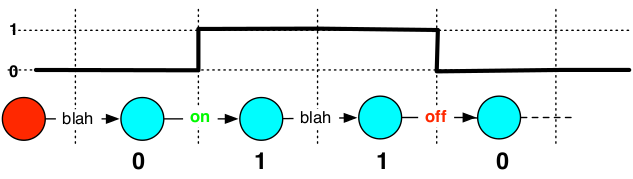
\includegraphics[width=6cm]{fluent.png}
    \\
    \end{tabular}
    \caption{Propositional fluents changes with sets of
    initiating and terminating actions}
\end{figure}

\subsection{Linear Temporal Logic}
A temporal logic is defined in two steps:

\begin{itemize}
    \item From traces (sequences of actions) to fluents(boolean variables)
    \item From fluents to temporal formule (assert)
\end{itemize}

The linear  temporal logic is interperted  over \textbf{infinite traces}
which means there  are \textit{no terminal states} (Without: END,  STOP, ERROR).

\paragraph{  } If  the  model  have terminate  state,  we  can make  them
non-terminal by looping on themselves.
(Example : Action \textit{done} on the terminal state.)

\subsection{The until operator}

$\varphi_1 U \varphi_2$ is true in state q \textcolor{red}{IFF} $\varphi_2$ is true in some future
state q' \textcolor{red}{AND} $\varphi_1$  is true in all states from q  to q' not included.

\begin{figure}[h]
    \centering
    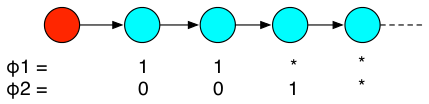
\includegraphics[width=6cm]{until.png}
    \caption{Until operator}
\end{figure}


In the example below, it means that we can't have enter before knock and
knock will happen.

\begin{lstlisting}
    assert POLITE1 = (!enter U knock)
\end{lstlisting}

\subsubsection{Semantics}

\begin{itemize}
    \item Interpretation over fluent $W_i$ = ($f_i, f_{i+1}, \cdots$) the $i^{th}$ suffix of w.
    \item Each $f_i \in 2^{\phi}$
\end{itemize}

$ W_i \textrm{ sat } \varphi \cup \varphi' \textrm{ \color{red} IFF \color{black} there is} \quad j \geq i
\textrm{ such that} \quad w_j \textrm{ sat } \varphi' \textrm{ and for all } i\leq k < j \textrm{ we have } w_k \textrm{ sat }  \varphi$


\subsection{Branching temporal Logic}

FTL is  limited as  it can only  distinguish trace-based  properties, we
can't for example distinguish proterty  on non-determinism (slide 37 cha
8.a).

Instead of considering trace, \textbf{Branching temporal logic} consider
execution tree.  There are  two types  of formula:  path and  state. The
quantifier are the following:

\begin{itemize}
    \item $\mathbf{AX \varphi}\equiv$ in all next state, $\varphi$ holds
    \item $\mathbf{EX \varphi}\equiv$ in some next state, $\varphi$ holds
    \item $\mathbf{E(\varphi U\varphi'} \varphi) \equiv$ there exists a path where $\varphi$ holds until $\varphi'$ holds
    \item ...
\end{itemize}

\begin{lstlisting}
P1 = (a->(b->STOP|c->STOP))
P2 = (a->b->STOP|a->c->STOP)
// ct1 CANCHOOSE = AX(a->EX b) //not in LTSA
\end{lstlisting}

This  property state  that we  can  choose between  b  and c.  As P1  is
deterministic, it  satisfied the  property but not  P2 because  a choice
cannot be done.

\section{Question 13: Temporal logic operator}

\textit{Using  small  examples,  explain  the  five  temporal  operators
of  FLTL (eventually,  globally,  strong and  weak  until, next).  Using
equations, show how [] and $<>$ derive from U and W and how U and W relate
to  each other.  State  and  explain the  expansion  law  for the  until
operator. }

\subsection{Example for operator}
\begin{description}
    \item[Globally :] []$\varphi$ is true in some state \textcolor{red}{IFF} $\varphi$ is true in that state and all future state.
    \item[Eventually :] $<>$ $\varphi$ is true in some state \textcolor{red}{IFF} $\varphi$ is true in that state or in some future state.
    \item[Strong until :] $\varphi_1 U \varphi_2$ is true in state q \textcolor{red}{IFF} $\varphi_2$ is true un some future state q'
    \textbf{and} $\varphi_1$ is true in all states from q to q' not included.
\item[Weak until (unless) :]  $\varphi_1 W \varphi_2$ is true in state q \textcolor{red}{IFF} $\varphi_1$ is true in all states from q as
    long as $\varphi_2$ is false.
\item[Next :] X $\varphi$ is true in some state \textcolor{red}{IFF} $\varphi$ is true in the next state
\end{description}

\begin{lstlisting}
fluent CRITICAL[i:1..N] = <p[i].enter,p[i].exit>

// Globally
assert MUTEX = []!(CRITICAL[1] && CRITCAL[2])

// Eventually
assert LIVE = <>(CRITICAL[1] || CRITICAL[2])

// Strong until (knock must happen)
assert POLITE1 = (!enter U knock)

// Weak until (knock can happen)
assert POLITE2=(!enter W knock)

// Next
assert QUICK = (p[1].enter -> X p[1].exit)
\end{lstlisting}

\subsection{Relation between operators}

$<>$ and [] are particular cases of U and  W. At the same time U and W are
related. The differents relations are the following.

\begin{eqnarray*}
<> \varphi &=& \quad  true \quad U \varphi \\
\textrm{[ ] } \varphi &=& \varphi W \quad false \\
\varphi W \varphi' &=& \varphi U \varphi \quad || \quad \textrm{[ ] } \varphi \\
\varphi U \varphi' &=& \varphi W \varphi' \quad\&\& \quad <> \varphi
\end{eqnarray*}


\paragraph{Can be reduced to}
U and [] or W and $<>$

\subsubsection{Law duality U-W and []-$<>$}

\begin{eqnarray*}
! (\varphi U \varphi') &=& ! \varphi ' W (!\varphi \quad \&\& \quad !\varphi ') \\
! (\varphi W \varphi') &=& ! \varphi ' U (!\varphi \quad \&\& \quad !\varphi ') \\
\\
! [] \varphi &=& <> \quad! \varphi \\
! <> \varphi &=& [] \quad! \varphi
\end{eqnarray*}

\paragraph{ } So duality can be reduced by using !

\subsection{Expansion of Law}

\textbf{Expansion  law}  unrolle  operators  on  step,  for  the  until
operator, the expansion is as follow

$$\varphi U\varphi' = \varphi'\quad || \quad (\varphi \quad \&\& \quad X (\varphi U \varphi'))$$

\section{Quesiton 14: Model-checking principle}

\textit{Explain the general  principles of automata-based model-checking
of  linear temporal  logics. Discuss  the cases  of safety  and liveness
properties. Define the notion of  Büchi automaton. Explain what results
are produced.}

\paragraph{Naïve idea}
\begin{enumerate}
    \item Turn a LTL property $\varphi$ into a property automaton $B_{\varphi}$
        so $B_{\varphi}$ reaches ERROR when $\varphi$ is violated
    \item Build ($B || B_{\varphi}$)
    \item Apply reachability algorithm to search for ERROR
\end{enumerate}

Don't work because we need to use \textit{infinite traces} for liveness properties.
(reachability is only on finite trace)

\subsection{General principle}
We have three set for the language

\begin{itemize}

    \item L = $(\alpha  B)^\omega$ where B is a model  and $\alpha B$ it
    the  alphabet.  It  represents  the universal  language  of  B,  all
    possible infinite traces. ($\omega$ is denumerable infinity)

    \item L(B)  =$\{ \sigma \in  L | B =  \sigma=>\}$, the language  of B
        (\textit{set of execution traces}). Attention, there is the assumption that B
    has no finite terminating execution.

    \item $L(\varphi) =  \{\sigma \in L|\sigma sat \varphi\}$  the language of
    $\varphi$ (\textit{set of satisfiying traces}).

\end{itemize}

\subsubsection{Verification}

\paragraph{The goal} is to verify than B sat $\varphi$ :
\begin{enumerate}
    \item \textcolor{red}{IFF} for all (infinite full) traces $\sigma$ of B, $\sigma$ sat $\varphi$
    \item \textcolor{red}{IFF} L(B) $\subset$ L($\varphi$)
\end{enumerate}

It's not easy to verify, but there is another way.

\paragraph{Solution } To  see if  B  satisfy the  property  $\varphi$ we're  going  to check  the emptiness of L(B)  $\bigcap$ L(!$\varphi$).


\subsubsection{Synchronization}
Generally, synchronization produces the intersection of traces on the shared alphabet :

Given two LTS $B_1, B_2$ with A = $\alpha(B_1) \cap \alpha(B_2)$ :
$$ L(( B_1 \quad || \quad B_2) @ A) =  L(B_1 @ A) \cap L(B_2 @ A) $$
( @ show only this action )

\paragraph{Particular :} if $\alpha(B_1) = \alpha(B_2)$ then $L(B_1 || B_2) =  L(B_1) \cap L(B_2)$
\subsection{Automata-Based Model Checking}
To check the emptiness of L(B) $\cap   L(!\varphi)$, we will do as follow:

\begin{enumerate}
    \item Build an automaton $B_{!\varphi}$ with same alphabet as B which accepts $\sigma$ such that $\sigma$  sat !$\varphi$

        (\textit{Need Büchi automata to solve infinite trace problem})
\item Compose $B || B_{! \varphi}$
    \item Search for a trace $\sigma$ accepted by $(B||B_{!\varphi})$

    (\textit{Need SCC and terminal sets to solve the problem of reachability with infinite trace})
\end{enumerate}

If $\sigma$  can be found,  it means  that is trace  of B that  does not
satisfy the  property $\varphi$, it's  therefore an  error trace and  so B
does not satisfy $\varphi$


\subsection{Model Checking for Safety and Liveness property}
Given a (LTS) model B and a property $\varphi$,
verify that B sat $\varphi$.

\begin{itemize}
    \item To check if a model is \textbf{deadlock freedom} we check the \textit{reachability} of deadlock state
    \item To check a \textbf{safety property} we check the \textit{reachability} of ERROR state
    \item To check a \textbf{progress propety} we check the possible action in \textit{terminal sets}
    \item To check \textbf{LTL propeties} we check the \textit{reachability of accepting state repeativly.}
\end{itemize}

\paragraph{Safety} use juste reachability algorithm to have the result

\paragraph{Liveness} is more  complicate because the search  are done on
infinite  trace, reachability  is not  enough, we  use Strong  connected
component or terminal sets.

\subsection{Büchi automaton}

\begin{figure}[h]
    \centering
    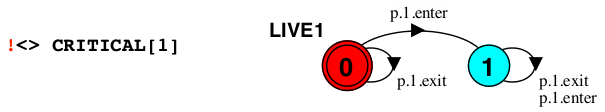
\includegraphics[width=10cm]{buchi.png}
    \caption{Automaton example}
\end{figure}

Büchi automaton are  automaton with states marked  as accepting states.
This kind of  automaton accepts infinite traces that  visit an accepting
state infintely often and is generally non-deterministic.

The verification  is done on  the following relation, accepting  trace =
error trace.

A  Büchi automaton B is  a quintuple $B = <S,\Sigma,\Delta,q,F>$ where

\begin{itemize}
    \item S is a finite set of states.
    \item $\Sigma$ is a finite set of symbols.
    \item $\Delta \subseteq Sx\Sigma xS$ is a labelled transition relation.
    \item $q\in S$ is an initial state.
    \item $F\subseteq S$ is a set of accepting state.
\end{itemize}

\textbf{B  accepts an  infinite  trace $\sigma  = (a_0,a_1,a_2,...)  \in
\Sigma^\omega$  \textcolor{red}{IFF} there exists an infinite execution over $\sigma$ that
visits  F infinitely  often.}


\paragraph{LTL to büchi}
It  is possible  to translate  LTL formula
$\phi$ on alphabet A into Büchi automaton $B_{!\phi}$ over $\Sigma=2^A$
such that  $B_{!\phi}$ accepts $\sigma$ \textcolor{red}{IFF} $\sigma$ sat  $!\varphi$.

\subsubsection{Example}

\begin{figure}[h]
    \centering
    \begin{tabular}{cc}
        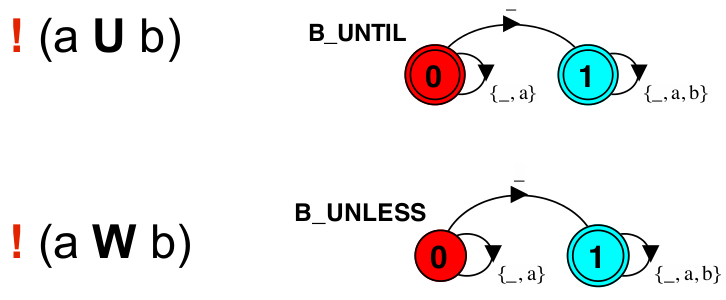
\includegraphics[width=8cm]{buchi_ex1.png}&
        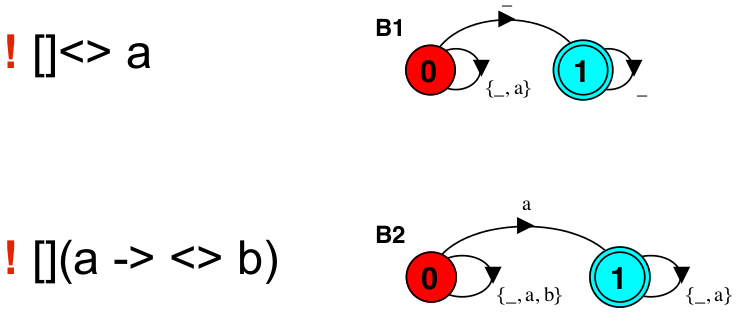
\includegraphics[width=8cm]{buchi_ex2.png}\\
    \end{tabular}
    \caption{Example of buchi automata}
\end{figure}


\paragraph{Result}
The accept trace is a error trace of the property $\varphi$.

\section{Question 15: Model-checking algorithm}

\textit{Discuss  the  algorithms  needed to  verify  deadlocks,  safety,
progress  and general  LTL properties.  Give the  general principles  of
these algorithms. Explain the double DFS algorithm and its complexity}

\subsection{Algorithms and principle}

\begin{itemize}
    \item To check if a model is \textbf{deadlock freedom} we check the \textit{reachability} of deadlock state
    \item To check a \textbf{safety property} we check the \textit{reachability} of ERROR state
    \item To check a \textbf{progress propety} we check the possible action in \textit{terminal sets}
    \item To check \textbf{LTL propeties} we check the \textit{reachability of accepting state repeativly.}
\end{itemize}

\subsection{General  principle for reachability algorithm : }
Given a  LTS $<S,A,\Delta,q_0>$  return a state  q statisfying  c(q) and
reachable from $q_0$, otherwise fail

\begin{lstlisting}
REACHABLITY(lts,c):
	close :={} //keep track of visited state
	fringe :={q0}
	forever do
		if fringe ={} then fail
		q:= CHOOSE(fringe)
		if c(q) then return q  //with trace from q0
		if q not in closed then
			closed := closed U {q}
			fringe := fringe U {q'|q-a->q'}
\end{lstlisting}

\begin{itemize}
    \item Keep track of already visited states (closed) for \textbf{efficiently}
    \item Strategy choose the next state

    \item   Depending   on   how   the  fringe   is   handle,   it's   a
    \textcolor{red}{DFS}  (fringe as  stack)  or a  \textcolor{red}{BFS}
    (fringe as a queue).
\end{itemize}


\subsubsection{Verification}
\paragraph{For deadlock:}c(q)  $\equiv$ q has no  outgoing transitions.

\paragraph{For safety properties:}c(q) $\equiv$ q is(or contains) ERROR.

\paragraph{ }\textbf{Successful} reachability = \textbf{failed} verification

\subsection{General principle for SCC algorithm : }
The input is a LTS B and the output is the set of SCCs of B

\begin{enumerate}
    \item Perform a depth-first search from $q_0$
    \item Each state q has two label
    \begin{itemize}
        \item index[q] = sequential index assigned in DFS order
        \item lowlink[q] = index of state reachable from q and $\le$ index[q]
    \end{itemize}
    \item State are accumulated on a SCC stack during the search
    \item if index[q] =lowlinl[k] after exploring q
    \begin{itemize}
        \item q is the root of an SCC in the DFS search tree
        \item The states of the SCC are on the SCC stack up to q
        \item The path to SCC is the DFS stack
        \item Terminal SCC is not backtracking from earlier SCC
    \end{itemize}
\end{enumerate}

\subsubsection{Example}
TODO add or explain example beginning  at slide 25 chap 8b.

\subsubsection{Verification}

\paragraph{Progress properties}
The  progress property  are checked  on the  SCC.
\begin{enumerate}
    \item Search for SCCs
    \item Check that each terminal SCC contains at least one action of
          each progress property.
      \item If not, report path to SCC and alphabet of SCC
  \end{enumerate}

\paragraph{LTL properties}

To verify that B sat $\varphi$, check that L(B) $\cap$ L($! \varphi$) = $\emptyset$.

\begin{enumerate}
    \item Buil büchi automaton $B_{!\varphi}$
    \item Compose ($ B || B_{!\varphi}$)
    \item Search(infinite) accepting trace in $(B||B_{!\varphi})$.
\end{enumerate}

Hard because seach for \textit{infinite traces} but $B || B_{!\varphi}$ is \textit{finite}

The  goal to achieve  that is  to find a  lasso shaped
trace with an accepting  state on the loop.
($\sigma = \sigma_1 \sigma_2^{\omega} $ where $\sigma_1, \sigma_2$ ar finite)

We can do that by using the SCC algorithm or the double DFS.

\subsection{Double DFS algorithm}
Given a Buchi automaton B = $<S,\Sigma,\Delta,q_0,F>$, return true \textcolor{red}{IFF} B has an accepting trace.
\begin{lstlisting}
DDFS(B):
	closed1 := {}
	closed2 := {}
	DFS1(q0)
	return false

DSF1(q)
	closed1 := closed1 U {q}
	for all q'|q-a->q' do //all succesors of q
		if q' not in closed1 then DFS1(q')
	if q in F then DFS2(q,q)	// F is the set
                                        // Of accepting state

DFS2(q,q*)
	closed2 := closed2 U {q}
		for all q'|q-a->q' do
			if q'=q* then return true // with stack trace of DFS1 and DFS2
			else if q' not in closed2 then DFS2(q',q*)
\end{lstlisting}

\subsubsection{Example}
TODO add or explain example beginning  at slide 39 chap 8b.

\section{Question 16: Model-checking optimization}

\textit{Discuss the  complexity of  model checking  for LTL.  Define the
notion of  independent transitions, and  explain how  it can be  used to
optimize model-checking. Explain the  principles of bitstate hashing and
discuss its impact on model-checking.}

\subsection{Complexity}
\begin{itemize}
    \item $| \quad B||B_{!\varphi} \quad |$  =  O($|B|\times|B_{!\varphi}|$) where  $|B|$  is number  of transition in B.
\end{itemize}

The complexity is \textbf{linear} with respect  to the sizes of
the LTS and automaton but it's \textbf{exponential} in the size of the FSP model
(\textcolor{red}{state-space} explosion)

\begin{itemize}
    \item Indeed, $|B!\varphi|$ =  O($2^{|\varphi|}$) (each value in the  formula can be
true  or false)  =$>$  exponential in  the  size of  the  LTL formula.
\end{itemize}

\subsubsection{In pratice}
The size  of  the model  is the  big  factor, because  formula
remains relatively small.

\subsection{Fighting state-space explosion}
There is different solution :

\begin{enumerate}
    \item Avoid exploring redundant executions (\textbf{partial-order reduction})
    \item Merge similar states (We don't see this part)
    \item Partial model-checking (\textbf{bitstate hashing} and guided search not see
        in this part)
\end{enumerate}

\subsection{Independent Transition and Optimization}

To reduce the state-space explosion, we try to avoid exploring redundant
execution  by partial  order reduction,  it's in  this context  that the
notion of  independent transition is important.

\textbf{Partial order reduction} consists of three things:

\begin{enumerate}
    \item{Independency :} Two transition q-a-$>$q',q-b-$>$q'' are independent \textcolor{red}{IFF} there is a state q''' such that q''-a-$>$q''' and q'-b-$>$q'''

       (\textit{Hard to determine without exploring full graph})
    \item{Invisibility :} A transition q-a-$>$q' is invisible with respect to a property $\varphi$ \textcolor{red}{IFF} it does not affect the  value of $\varphi$

        (\textit{Action don't change de fluent value})

    \item{Ample set :} A set A of enabled actions such that
    \begin{itemize}
        \item A is not empty unless there is no enabled action.
        \item Any execution of action other than A from q contains only actions that are independent from actions in A
        \item Action in A are invisible with respect to the verified property unless A contains all enabled actions
        \item On any cycle , an enabled action is not ignored indefinitely
    \end{itemize}
\end{enumerate}

\begin{figure}[h]
    \centering
    \begin{tabular}{cc}
        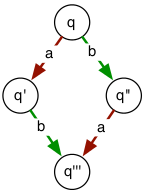
\includegraphics[height=3cm]{independant.png}
        &
        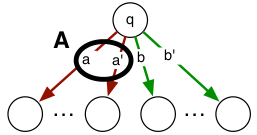
\includegraphics[height=3cm]{ample.png}
        \\
        Independency & Ample set \\
    \end{tabular}
    \caption{Partial order reduction}
\end{figure}


\subsubsection{Fonctionnement}

Partial  Order Reduction  consits  in exploring  only  ample sets,  they
are  used  to  reduce  the   number  of  interleavings  explored  during
model-checking.

\subsection{Bitstate hashing}

Let \textbf{h} be  the size of a hashtable and  \textbf{r} the number of
state stored in the hashtable.

If keep $r<<$h,  most state have a unique  hash code (\textcolor{red}{no
colision}). With Bistate  Hashing, insteaf of keeping the  full state in
the hashtable,  we only have  very large hashtable that  contains single
bits.

When we want to  add a state q, we simply set h(q)  to 1.

The  problem  is  that  if  there   are  collision  some  state  can  be
\textbf{missed} but the probability is low if r $<<$ h.

\paragraph{ }
With \textbf{bloom filters} where  we set k
bits per states(in  different cells), the number of  collision is reduce
but the table fills k times more quickly.

\section{Question 17: Petri nets }

\textit{Using a  small example,  explain the  structure and  dynamics of
Petri  nets. Formalize  their  semantics in  mathematical terms.  Define
reachability and  coverability of  states. Explain the  construction and
usage of the coverability tree. }

\subsection{Structure of PN}
\begin{figure}[h]
    \centering
    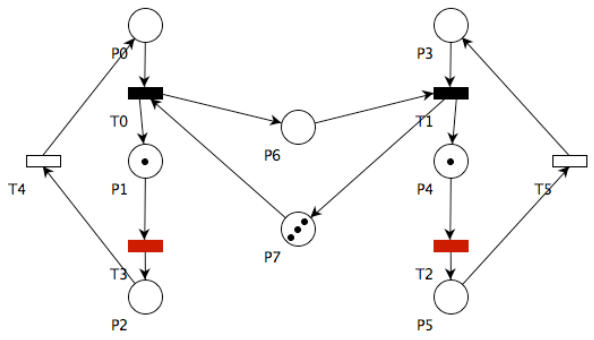
\includegraphics[width=10cm]{petri.png}
    \caption{Petri-net example}
\end{figure}

A petri net is a bipartite graph. It's composed of:
\begin{itemize}
    \item Place $\bigcirc$ which represents a condition
    \item Transition $\arrowvert$ which represents an event
    \item Arc $\to$ that relate event to transition.
        \begin{enumerate}
            \item place-transition arcs = input = required
            \item transition-place arcs = output = resulting
        \end{enumerate}
\end{itemize}

The structure of a petri net graph is as follow $$N = <P,T,A,w,x>$$ where

\begin{itemize}
    \item P is a finite set of places
    \item T is a finite set of transitions
    \item $A \subseteq(PxT)\bigcup(TxP)$ is a finite set of arcs
    \item $w:A\to N_0$ is the weight function on the arcs
    \item $x:P\to N$ is a marking or state (the number of tokens in each place)
\end{itemize}

\begin{figure}[h]
    \centering
    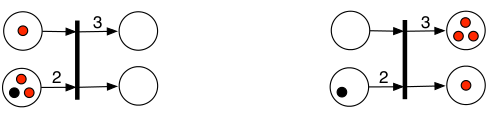
\includegraphics[width=5cm]{weight.png}
    \caption{Arc weight}
\end{figure}

When a  tranistion is  triggered, the  number of  token in  the incoming
places  of  the transition  are  moved  to  the  outgoing place  of  the
transition according to the weight of the arc (incoming and outgoing).

A  transition can  only be  trigger  if there  are enough  token in  the
incoming place compared to the weight of the arc.

\subsection{Semantics of PN}
\label{petri}
\paragraph{Place, transition and marking} are represented as vector:

\begin{itemize}
    \item P = [p1,p2,...pn]
    \item T = [t1,t2,...,tn]
    \item x = [x(p1),x(p2),...,x(pn)]
\end{itemize}

\paragraph{ } For a  transition t $\in$ T,
\begin{eqnarray*}
    \bullet t = I(t)  &=& {p \in P  |(p,t) \in A} \textrm{ are the  input places of t }\\
    t\bullet=O(t) &=& {p\in P|(t,p)\in A}\textrm{ are the  output places of t }
\end{eqnarray*}

(same thing can be done  for the place).

\paragraph{ }  Given a  petri net N=(P,T,A,W,x),  \textbf{the transition
function} $f:N^nxT\to N^N$ is a partial fucntion defined as
\begin{itemize}
    \item f(x,t) is defined \textcolor{red}{IFF} $\quad \forall p \in \bullet  t,x(p) \geq w(p,t)$
    \item if f(x,t) is  defined, \textcolor{red}{THEN} f(x,t) = x' where  $ \quad x'(p) =  x(p)-w(p,t)+w(t,p)$
\end{itemize}

\subparagraph{Attention},  it means  that  the number  of  token is  not
always constant.

\subsection{State equation}
$$ x' = x + u A$$


\subsection{Reachability}

\subsubsection{Reachable state space}
For a \textit{sequence of transition} $\sigma \in T*$ :
\begin{eqnarray*}
    f(x, \epsilon) &=& x\\
    f(x, \sigma t) &=& f(f(x, \sigma), t)
\end{eqnarray*}

\paragraph{ }
\begin{description}
    \item[Reachable state space R(n) $\subseteq$ N] for a given Petri net N = (P, T, A, w, x) :
        $$R(N) = {x' \in N^n  \quad| \quad \exists \sigma \in T*,f(x, \sigma=x')}$$
        (it means all the state marking reachable from x through transition in T)

    \item[Reachability :] given a trajectory equation, a state x' is reachable from x
        \textcolor{red}{IF} $x = \sigma\Rightarrow x'$ with $\sigma$ a sequence of transitions.

        If this is \textbf{true} then there is a firing count vector v such a $$\textrm{vA = x' – x}$$
    Implication in one way only but, if no solution then x' not reachable.
\end{description}

\subsection{Coverability}

\begin{description}
    \item[State coverage]: A state x covers a state y $(x \geq y)$ \textcolor{red}{IFF}
        $$ x(p) \geq y(p) \quad \forall p \in P$$

        The coverage state space grows \textit{monotonically} with the initial marking

    \item[Coverability: ]A state x is coverable in Petri net N \textcolor{red}{IFF}
        $$ x\leq y \quad \textrm{for some} \quad y \in R(N) $$
\end{description}

Coveraibility is an approximation of reachability.


\paragraph{ } For a transition $ t \in T, let pre(t) = [w(p_1, t), \cdots, w(p_n, t)]$
t \textbf{can be fired} in a preti net \textcolor{red}{IFF} pre(t) is \textbf{coverable} in N


\subsubsection{Construction coverability tree}

\paragraph{Principe} : Group all nodes  [1 0 \textcolor{red}{k}] for all
k under a signe node [1 0 $\color{red}\omega$]

(If we have [1 0 0] and [1 0 1]  on the same path, we will have [1 0 2],
[1 0 3], \ldots)


\begin{figure}[h]
    \centering
    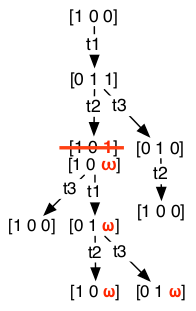
\includegraphics[width=4cm]{cove_tree.png}
    \caption{Example}
\end{figure}

\paragraph{Algorithm}

\begin{enumerate}
    \item Add $x_0$ to the new nodes
    \item WHILE there is a new node x

        \begin{enumerate}
            \item IF there is y = x on the path to x THEN x is a \textit{duplicate node}
            \item ELSE IF x has no enabled transitions THEN x i a \textit{terminal node}
            \item ELSE FOR each $x -t \to x'$

                \begin{enumerate}
                    \item add $x -t \to x'$ to the tree and add x' to the new nodes

                    \item IF x(p) = $\omega$ THEN set x'(p) = $\omega$
                    \item IF there is y $<$ x' on the path to x
                        THEN set x'(p) = $\omega$ for all p such that x'(p) $>$ y(p)
                \end{enumerate}
        \end{enumerate}
\end{enumerate}

\paragraph{Property}
\begin{itemize}
    \item Coverability tree of any petri net is \textbf{finite}
    \item Coverability tree \textbf{covers all states} in R(N)
\end{itemize}

\paragraph{For a coverability tree for a petri net N given} :

\begin{itemize}
    \item N is \textit{bounded} \textcolor{red}{IFF} no $\omega$ in the tree. (coverability tree = reachability tree)
    \item y \textit{coverable} in N \textcolor{red}{IFF} there is somme x $\geq$ y in the tree.

        (if x(p) = $\omega$ for somr p, then the path to x contains loops)
    \item $\gamma$ is \textit{conserved} by N \textcolor{red}{IFF} $x \omega^T = C$ for all x in the tree.

        ($\gamma(p) = 0$ fo all p such that x(p) = $\omega$ for some x)
\end{itemize}



\section{Question 18: Petri nets linear algebra}

\textit{Using a  small example,  explain the  structure and  dynamics of
Petri  nets. Develop  the matrix-based  representation of  Petri nets  :
incidence matrix,  trajectory equation,  firing count vectors.  Show how
this can be used to compute conservation and periodicity properties}

\subsection{Structure of PN}
See \ref{petri} page \pageref{petri}

\subsection{Matrix-Based Representation}

\begin{description}
    \item[Incidence matrix] $A=a_{ji}$ of size m x n such that $a_{ji} = w(t_j,p_i)-w(p_i,t_j)$

    \item[Trajectory Equation]: For a sequence of transitions
        $$\sigma=t^1...t^k\in T* \quad \textrm{such that} \quad x=\sigma \Rightarrow x'$$

        we have \textbf{x' = x+vA} where v is the firing vector (number of time that a transition is fired over $\sigma$)

    \item[Firing count vector] If x = $\sigma \Rightarrow x'$ then
        $$ x' = x + v A$$
\end{description}


\subsection{Conservation}
Puts lower-bound on \textit{combination} of places.

\begin{description}
    \item [Place-invariant] : vector of weights for the markings of places.
    \item [Weighted marking] : weighted initial marking regardless of firing count.
\end{description}

\paragraph{ }
Consider a \textbf{weighting vector} $\gamma = [ \gamma(p_1), \cdots, \gamma(p_n)]$,
a Marked Petri net N is \textbf{conservative} w.r.t $\gamma$ \textcolor{red}{IFF}
$$ \sum p\in P \quad \gamma(p) x(p) = x \gamma^T \quad \textrm{is a constant } C$$

\subparagraph{$\gamma$ is a \textbf{place-invariant} of N},
it's a property of graph independent of the initial marking.


\subsection{Periodicity}
Given firing count vector restores initial marking.
Transition invariant = firing count vector.

\paragraph{ }
A Marked Petri net N is \textbf{periodic} w.r.t v \textcolor{red}{IFF}
$$ f(x, \sigma) = x \quad \textrm{for all } \sigma \textrm{ whose firing count vector is v }$$

\subparagraph{v is a \textbf{transition-invariant} of N},
it's a property of graph independent of the initial marking.

\subsection{Compute}
Use the incidence matrix to compute.

\end{document}
